\section{Problem Definition}\label{sec:Problem Definition}
Is it possible to close to gap between a general-domain pre-trained convolutional neural network and an in-domain pre-trained convolutional neural network, through the use of different fine-tuning ideas?
\vspace{3mm}\\
For the purpose of investigating the problem definition, a previous study by \textbf{\textit{Ingwersen}}\autocite{Ingwersen} are used as threshold for the in-domain accuracies. The general-domain models proposed in this study are two convolutional neural networks pre-trained on the well known ImageNet dataset, and fine-tuned by training on a limited supervised in-domain dataset, originating from the \hyperref[sec:DRE19]{Danish housing market}. The domains of the general-domain and the in-domain are investigated to get an understanding of what learned features each model might possess.
\section{Introduction}\label{sec:Introduction}
The purpose of this study is to increase customer engagement with advertisements of real estate in Denmark. This should be done by helping people find apartments which are similar to other apartments they like. The main problem is to identify rooms with a similar feature vector in the "Danish Real Estate" dataset.
\vspace{3mm}\\
A previous study, by \textbf{\textit{Ingwersen}}\autocite{Ingwersen}, found that in-domain pre-training (Places365) of a CNN produced big improvements in image similarity compared to a general-domain model pre-trained with (Imagenet). The central question of this study is to investigate the capability of the general-domain to close the gap to the the in-domain model with only a small amount of in-domain labeled data. Ideas include fine-tuning different layers of the CNN, and an implementation of the supervised version of contrastive learning.

\subsection{The Problem Domain}
The average person in Denmark is moving a total number of six times during their entire life\footnote{https://www.boligsiden.dk/nyheder/2018/06/flyttestudie-vi-flytter-som-aldrig-foer/}. The process of moving  would by most people be equivalent to making a huge life decision. One obstacle home seekers will encounter is the overwhelming amount of houses on the market. Therefore filtering away uninteresting houses is crucial. This sound like an easy task for home seekers to overcome. However the filters available to the home seekers are very factual and only apply to hard constants like square meters, location and price.
\vspace{3mm}\\
A factor often considered essential when buying a home is the aesthetics of the home. Filtering for specific aesthetics is not available through any of the existing real estate agencies.
An easy solution for real estate agencies would be to add a parameter: \textit{Appeal} or \textit{condition}, rating from a scale of 1 through 10. This approach face more than one obvious problem:
\begin{enumerate}
  \item{Who should rate the homes?}
  \item{Everybody has different preferences}
\end{enumerate}
These two problems can be conquered by having the home seekers mark homes which matches their unique home aesthetics. Then a model, like the one proposed in this study, would be able to identify homes on the market, that matches the home seekers unique preferences. The models proposed in in this study calculates the similarity between images, by measuring the distance between the encoded representations produced by the general-domain models.

\subsubsection{Problem Solution}
Throughout the progress of this study, an in-domain dataset, which will be examined in \autoref{ExperimentalSetup}, has been available to study. The general-domain models used in this study will through fine-tuning the top layers with the in-domain dataset be able to learn representative feature vectors. By comparing the feature vectors it will be possible to differentiate images that are similar to each other from images that are dissimilar. This idea is already used by companies in other industries, like \texttt{Pinterest} shown below.
\begin{figure}[H]
    \centering
    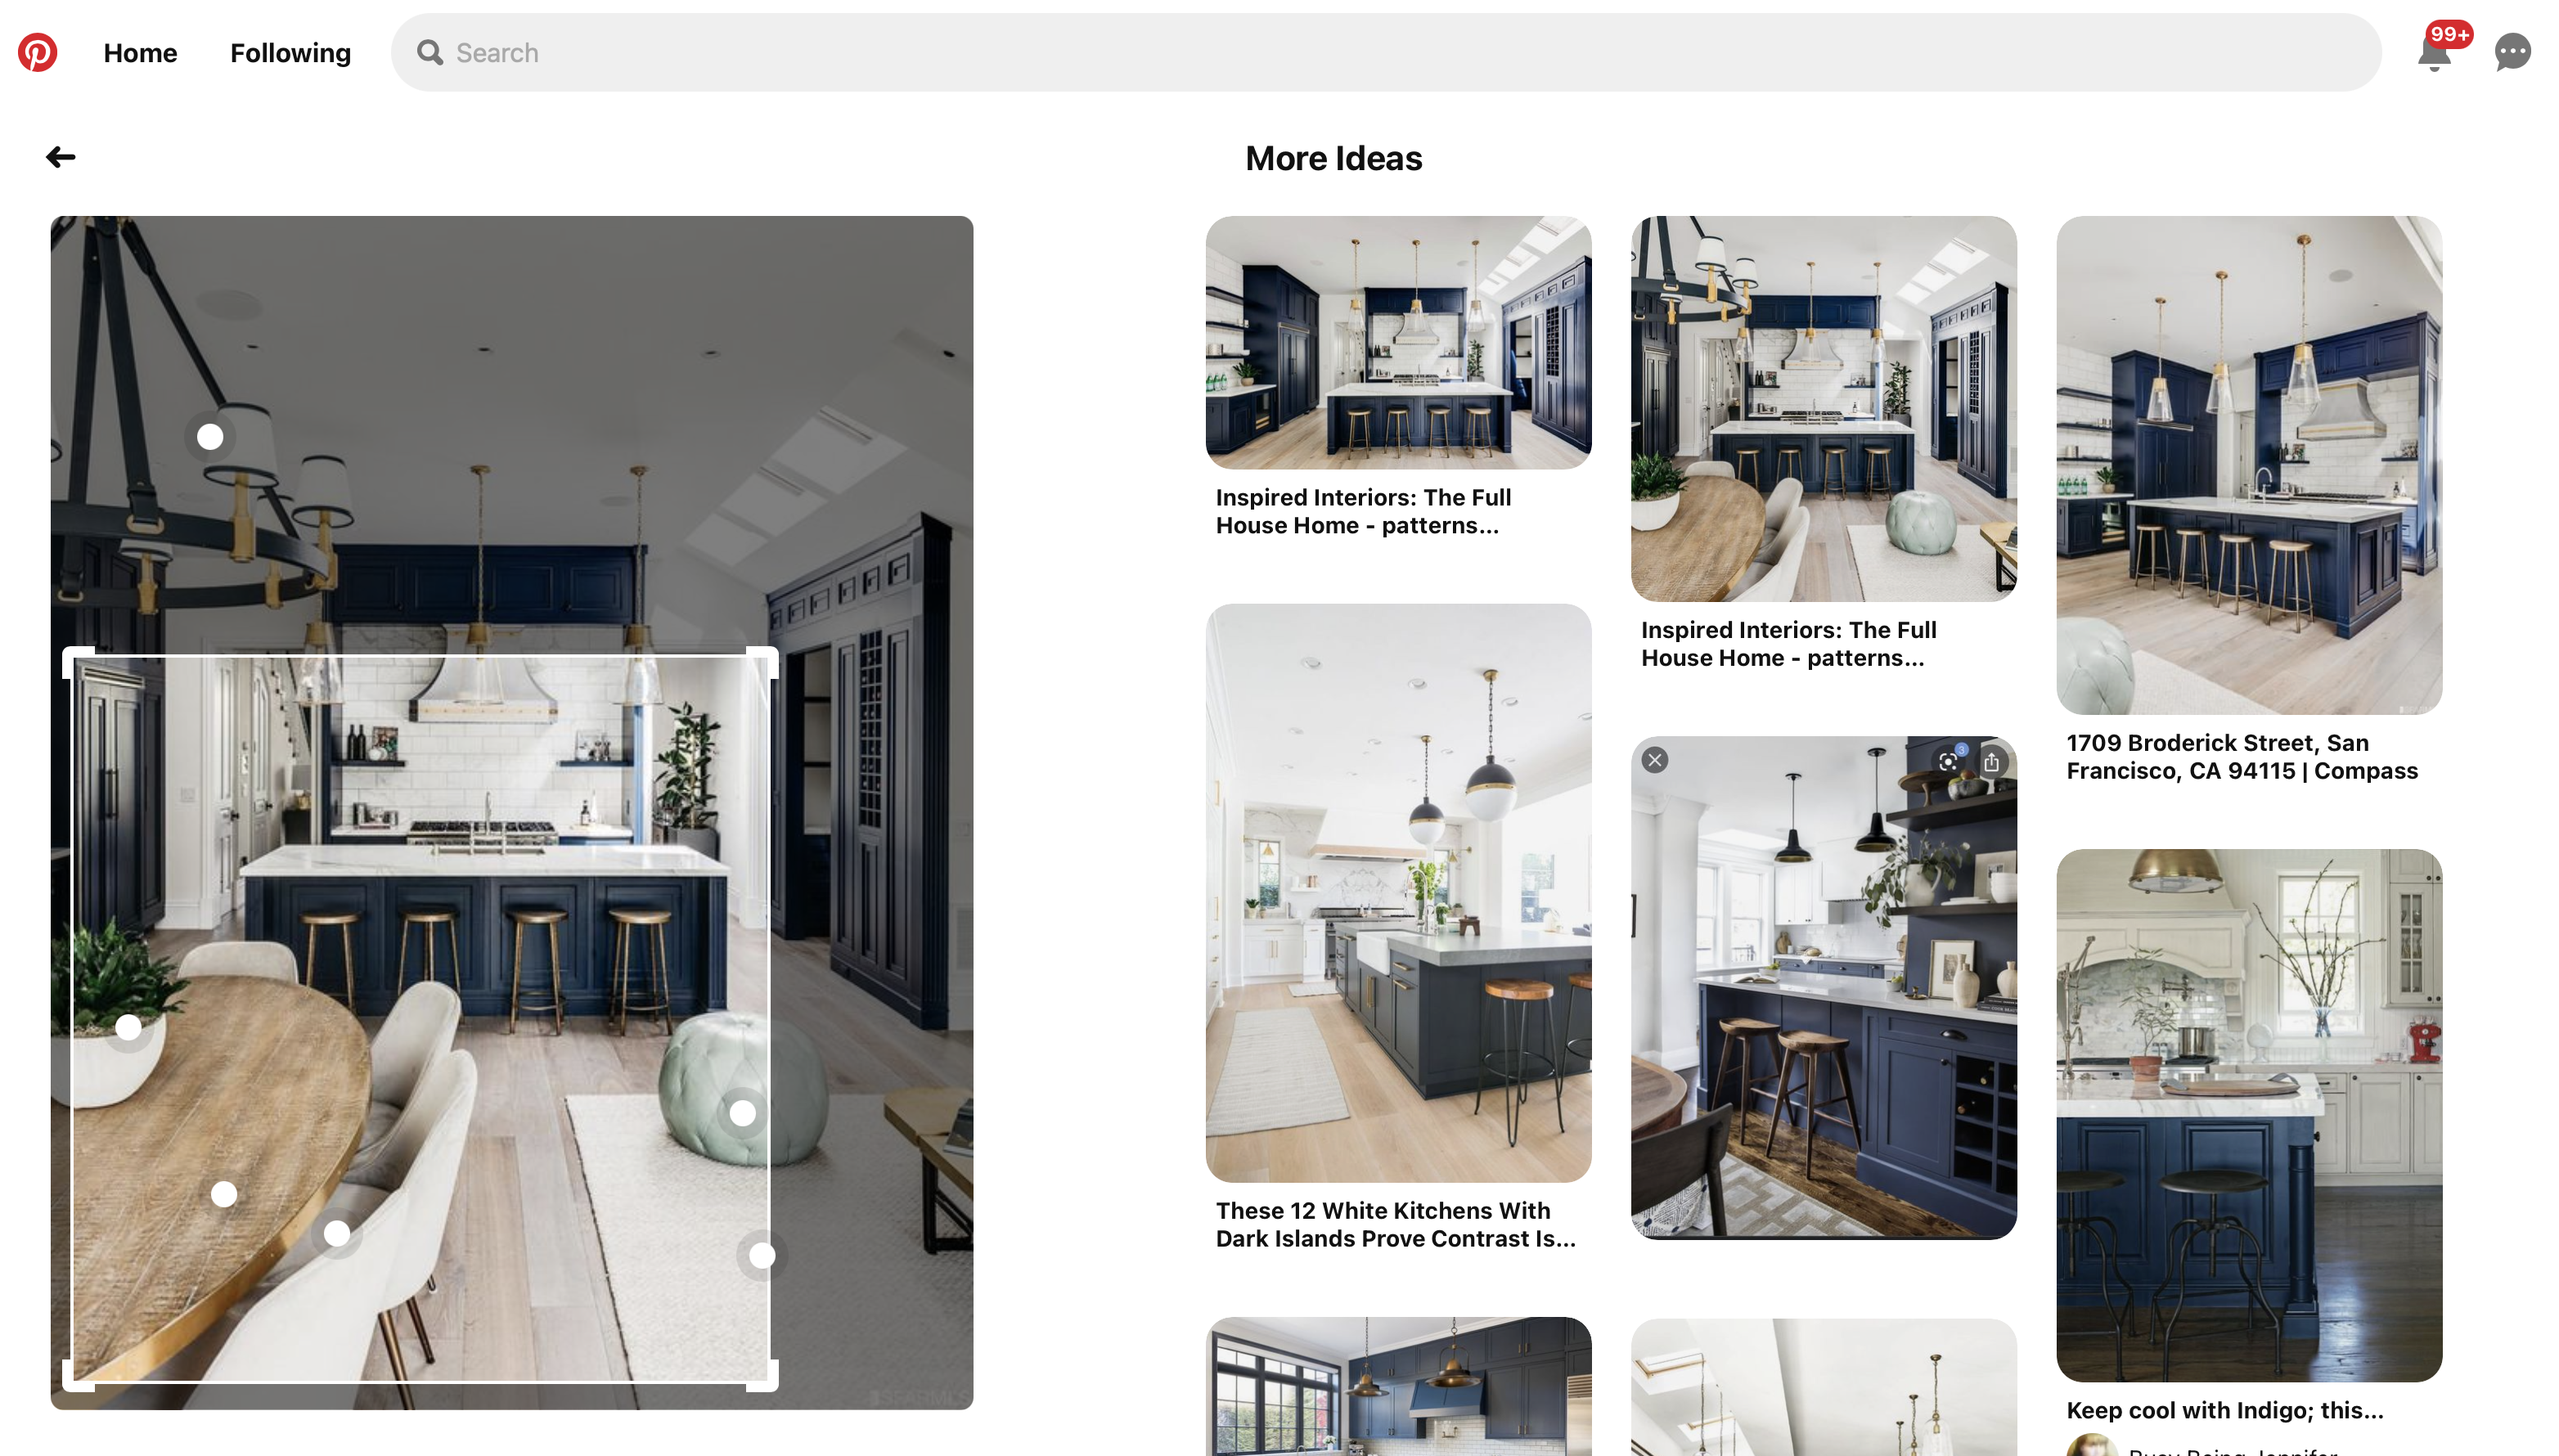
\includegraphics[scale=0.2]{pictures/random/pinterest}
    \caption{Pinterest Visual Similarity}
    \label{ref:pinterest}
\end{figure}
This study has implemented different models, which like \texttt{Pinterest} are able to measure similarities in images. \texttt{Pinterest} is a big company and has a lot of resources available, which are not available to any of the real estate agencies in Denmark. The models in this study is an attempt to fairly cheap, using limited data and publicly available libraries and pre-trained models, to implement a solution for capturing similarities in rooms, which is similar to the model used by \texttt{Pinterest}. As the results will show, this was a success.
